% !TEX encoding = UTF-8
% !TEX TS-program = pdflatex
% !TEX root = ../Tesi.tex
% !TEX spellcheck = it-IT

%************************************************
\chapter{Introduzione allo logica dello spazio}
\label{cap:spazio}
%************************************************

\vfill

\begin{flushright}{\slshape
  …sì, per cui una chiesa barocca ha sotto di sé, \\
  accessibile, una chiesa romanica, \\
  sotto la chiesa romanica una basilica paleocristiana, \\
  poi si scende ancora e c’è il mitreo romano… \\
  Questa è Roma. \\
  Però, invece, apparentemente Roma è appunto atemporale, \\
  sembra non offrire nulla; \\
  e gli accessi sono segreti, alla vera realtà di Roma. \\
  Quindi corrisponde assai bene allo stadio opaco dell’infanzia e dell’adolescenza, \\
  quando si è in preda a questa cosa strana che è il voler scrivere…} \\ \medskip
    --- G. Agamben
\end{flushright}

%\begin{figure}
%\centering
%\subfloat[Tetraedro inscritto in un cubo]
%{\includegraphics[width=.45\columnwidth]{tetrarec-cube}} \quad
%\subfloat[Spazio Tetraedrico]
%{\label{fig:tetracube}%
%\includegraphics[width=.45\columnwidth]{tetrarec-tetrahedron}} \\
%\caption[Spazio Tetraedrico]{Spazio Tetraedrico}
%\label{fig:tetratetra}
%\end{figure}

%discorso riverbero non come elaborazione dell'amplificazione ma come costruzione delle
%riflesioni ambientali. Le distanze hai 4 stone identisci cosi da dislocare gli altoparlanti
%facilmente. Posto simmetrico posto. Filmarmonica in

\section{Riverberi}

Nel descrivere il percorso di ricerca applicata allo spazio espressa in questa
tesi si può definire il duplice ruolo \emph{strutturale} del riverbero:

\begin{description}
	\item [riverbero \emph{struttura-architettonica}]
		come definizione dell'ambiente, custodia del rito e della pratica musicale;
	\item [riverbero \emph{struttura-musicale}]
		come descrizione di un ambiente, custodia dell'idea musicale, culla di risonanze
		ricercate nella scrittura, forzate nei gesti, particelle del rito celato nel tubo
		sonoro e nel suo sconfinamento architettonico.
\end{description}

Qui i riverberi architettonici, siano essi locali che generali, non acquisiscono funzione di elaborazione
di un suono amplificato. L'altoparlante non ha funzione di amplificazione ma di dimensionamento della forma
acustica della chiesa. C'è una dimensione spaziale di creazione, di sintesi e simbiosi acustica con lo strumento
che non assume mai funzione di elaborazione ma dialogo, relazione e riflessione.

La riflessione, qualità intrinseca del riverbero, è oggetto di analisi e sintesi poli-dimensionale. 

In un dialogo tra il muro architettonico virtuale e la sola voce acustica dello strumento,
nel territorio mono-dimensionale di un confronto con la diffusione elettroacustica
convenzionale, si rischierebbe la scissione dall'immagine riflessa.

\clearpage

Il rapporto-confronto tra la voce acustica dello strumento musicale e la polifonica reazione 
architettonica al canto deve poter essere descritta nello spazio come un elemento simultaneamente
\emph{poli-dimensionale} e \emph{tempo-variabile}. Solo in questo modo ci si può permettere
di collocare le due entità, ormai voci dello stesso canto, in due luoghi diversi
della sala da concerto ed ottenerne un unico e solido corpo sonoro, mosso e stazionario così
come nella nella culla dell'ambiente originario. 

\begin{figure}[h]
\centering
{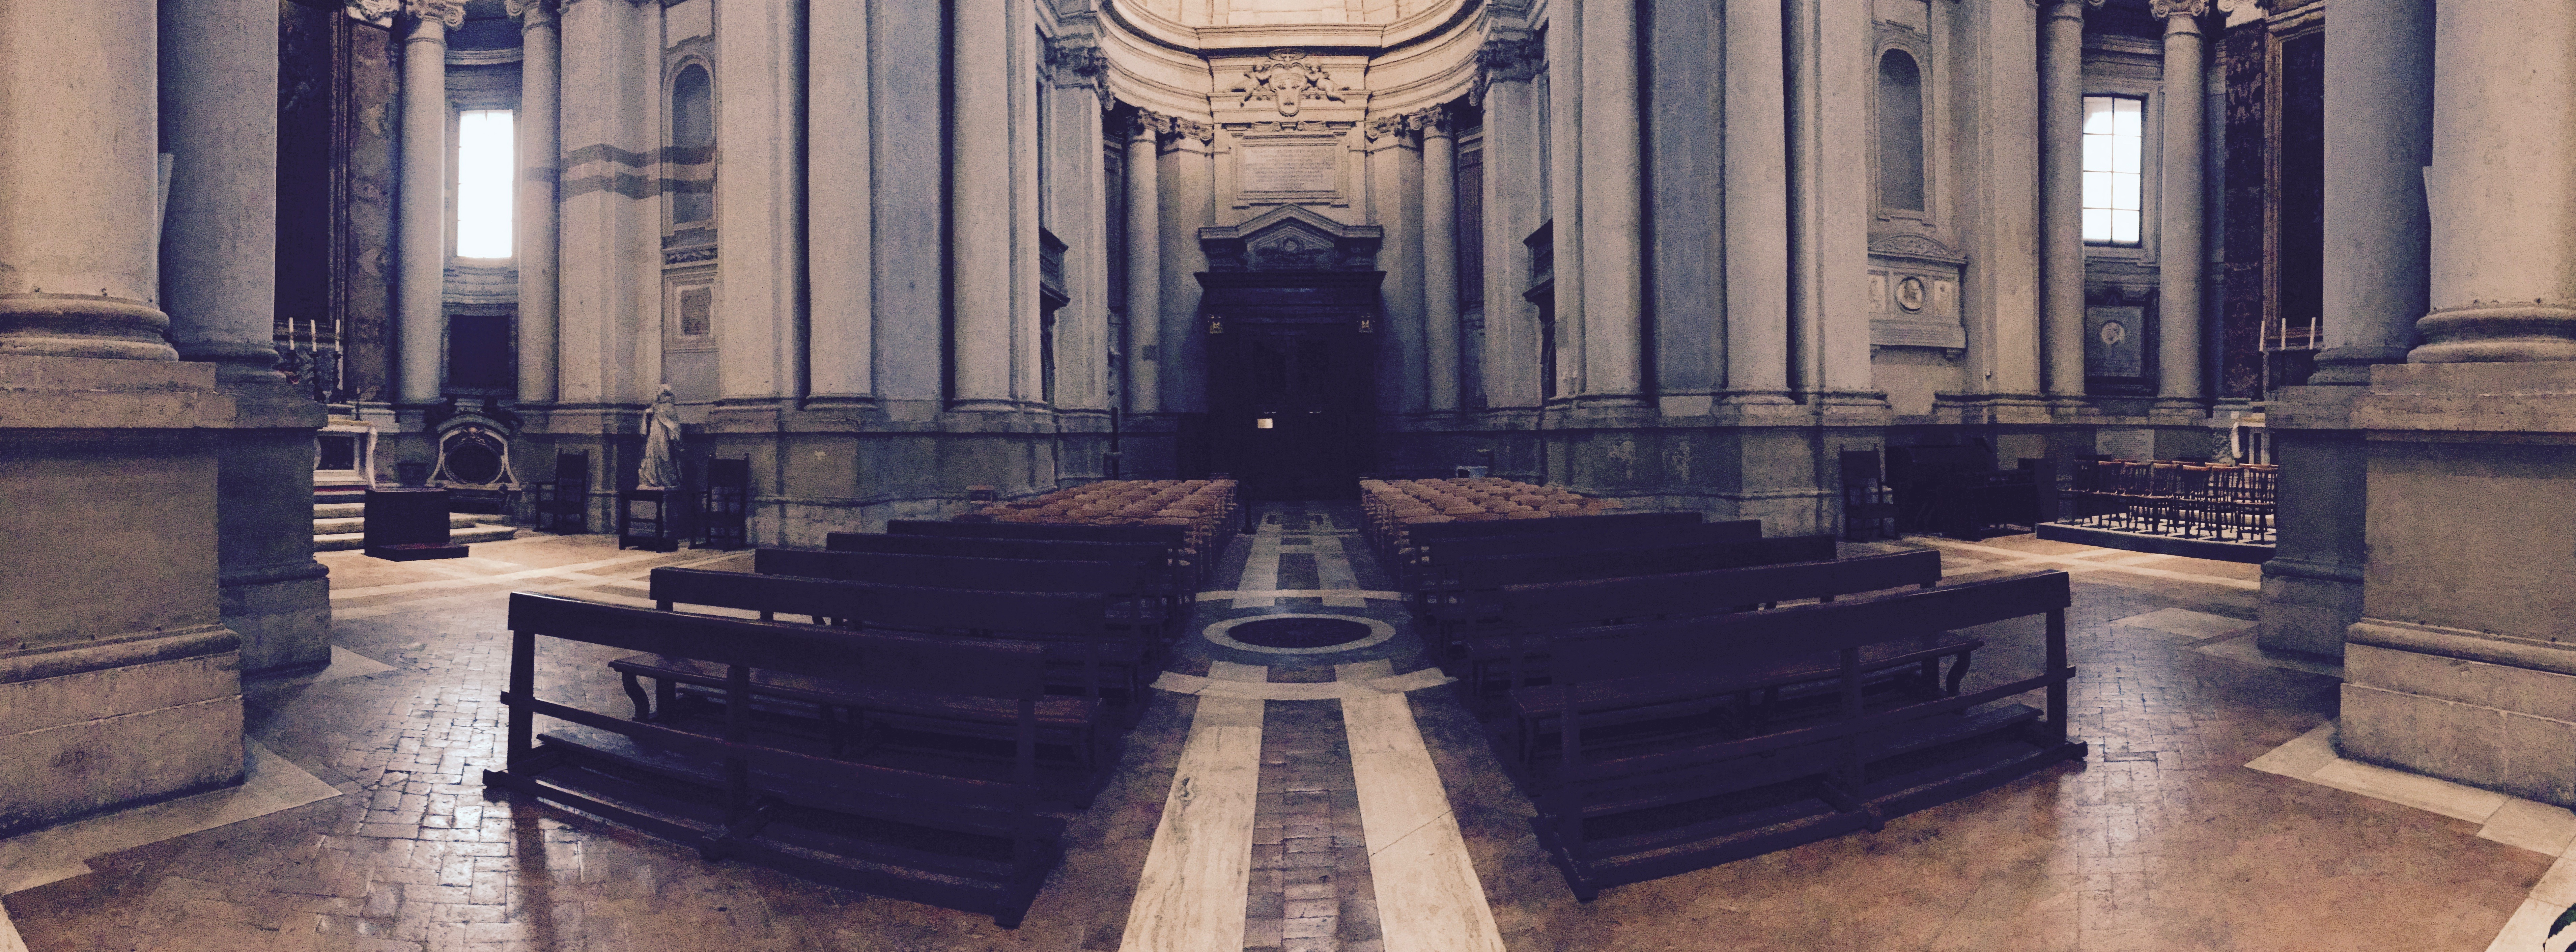
\includegraphics[width=.99\columnwidth]{ASM-IMG_3663}}
\caption[S. Luca, POV]{S. Luca, POV}
\label{fig:slucapov}
\end{figure}

La tecnologia elettroacustica è sussidio e consapevolezza di messa in scena funzionale alla
rievocazione del rito-luogo. La scelta del sistema elettroacustico \emph{S.T.ONE}\footnote{\emph{Spherical
Tetrahedral ONE}, diffusore elettroacustico composto di quattro facce triangolari per la riproduzione omni-direzionale
del campo sonoro} diviene elemento attivo nella stesura del brano sottoponendo elementi di dialogo strutturale, al tempo stesso
architettonico e musicale.

La scelta del numero minimo di diffusori, quattro, è volta alla ricerca della relazione di equilibrio tra
minima definizione tridimensionale e resa acustica in regime di verosimiglianza. Lo stesso Michael Gerzon
identifica in tre le sorgenti per la descrizione planare e quattro per la descizione perifonica.
Su questo principio si è operata una divisione dello spazio acustico descritto dalle mura in quattro regioni facilmente 
replicabili o identificabili in sala da concerto.

\section{Sistemi Elettroacustici}

Il progetto \emph{S.T.ONE} nasce dall'esigenza di poter eseguire musica elettroacustica,
sfruttando lo spazio sonoro creato dal mezzo elettronico, con caratteristiche percettive
acustiche analoghe a quelle degli strumenti tradizionali.

Un altoparlante tradizionale può essere controllato nella sola dimensione dinamica della
potenza e agendo su essa si può cercare un equilibrio con gli strumenti acustici.
Ma gli strumenti acustici hanno un comportamento molto più complesso, che implica relazioni
tra il fattore dinamico e quello timbrico e sopratutto spaziale del suono, creando uno
scollamento inevitabile tra ascolto acustico ed elettroacustico. S.T.ONE è il frutto di
una ricerca mirata alla soluzione di questo problema permettendo performance live in cui
la fusione tra i due soggetti, acustico ed elettroacustico, è totale, poli-dimensionale e completamente nuova all'ascoltatore. 

Con il diffusore S.T.ONE si può controllare la propagazione del suono riprodotto in tutte
le direzioni dello spazio e permettere di integrare questo controllo nei parametri della
composizione elettroacustica in un rapporto dialettico con lo strumento acustico.

L'ambizione è quella di superare un certo limite, identificato come appartenere intrinsecamente
all'oggetto altoparlante. L'oggetto, in quanto tale è stato il mezzo per giungere a quel limite e superarlo.

Il Limite. In un contesto di musica elettroacustica, ovvero di musica che si avvale parimenti
di oggetti acustici, strumenti tradizionali, oggetti elettrici ed elettronici, la diffusione
riprodotta dei suoni (mediante altoparlanti) ha sempre rappresentato un tema cruciale,
centrale per l'equilibrio acustico e musicale. Una buona integrazione tra suoni acustici
e suoni elettroacustici può tenere alta l'illusione di un unicum (ammesso che esso sia l'obiettivo)
ma è anche il varco attraverso cui introdurre il tarlo che farà crollare tutta la costruzione.
Questo ruolo di instabile funzionalità è si parametrabile all'ingegno che lo regola e lo dispone,
ma è anche dovuto al suo più grande limite: la direzionalità.

Un altoparlante nel migliore dei casi è un ottimo riproduttore di timbro e dinamica.
Ma l'elettroacustica ci ha insegnato che i parametri in gioco nella descrizione e
produzione di suono sono anche altri. La direzionalità, se vuole essere un parametro descrittivo,
deve poter variare nel tempo e non solo nella direzione di chi ascolta.

\vfill

\begin{figure}[h]
\centering
{\includegraphics[width=.99\columnwidth]{IMG_3529}}
\caption[Danilo Perticaro. \emph{S.T.ONE}.]{Danilo Perticaro. \emph{S.T.ONE}.}
\label{fig:dpstone}
\end{figure}
